% ============================================================
%  TERM PROJECT – PROPOSAL
%  Databases · THGA Bochum
%  Chess Club Tournament & Rating Manager
% ============================================================
\documentclass[11pt,a4paper]{article}

\usepackage{shared/thga-db}
\usepackage{caption}   % enables \captionof inside minipages
\graphicspath{{assets/}}

% ----- Placeholder figure (delete once you insert a real image) ----
\usetikzlibrary{positioning}
\newcommand{\placeholder}[3]{%
  \begin{tikzpicture}
    \node[draw=THGABlau!45, fill=THGABlau!5, very thick, rounded corners=2pt,
          minimum width=#1, minimum height=#2, align=center, inner sep=6pt,
          text=THGABlau!75, font=\small\itshape] {#3};
  \end{tikzpicture}%
}

% ----- Metadata --------------------------------------------
\renewcommand{\thgaKurs}{Databases}
\renewcommand{\thgaDatum}{Summer Term 2026}
\newcommand{\authorName}{Yahya El Idrissi}
\newcommand{\projectTitle}{Chess Club Tournament \& Rating Manager}

\begin{document}
\thispagestyle{empty}
\thgaTitel{Term Project -- Proposal}{\projectTitle}

\begin{infobox}
\textbf{Author:} \authorName \\
\textbf{Module:} Introduction to Database Management Systems · THGA Bochum \\
\textbf{Submitted to:} Stephan Bökelmann · \href{mailto:sboekelmann@ep1.rub.de}{sboekelmann@ep1.rub.de} \\
\textbf{Target size:} about 6 pages
\end{infobox}

% ============================================================
\section{Application domain and motivation}
% ============================================================

The project is a \textbf{Chess Club Tournament \& Rating Manager}: a small,
self-hosted system for managing chess-club tournaments, registrations, game
results, standings and Elo ratings in one persistent relational database.
Instead of keeping member data, tournament data and rating changes in separate
spreadsheets, the application stores the complete workflow centrally and keeps
current ratings and their history consistent. The system deliberately focuses
on tournament administration and rating management; automatic Swiss pairing
generation and advanced player-opening statistics are outside the final scope.

Two concrete usage scenarios illustrate the intended use:

\begin{itemize}[topsep=2pt]
  \item \textbf{Tournament director, Friday evening.} The director creates a
        tournament and specifies its number of rounds. The system automatically
        creates the corresponding round records, after which the director
        registers players, records game results and views the standings with
        points and Buchholz tiebreak values. Elo ratings are recalculated and
        stored immediately whenever a legal game result is recorded.
  \item \textbf{Club member or director, later.} The user opens the desktop
        frontend and reviews the current player list and Elo values, selects a
        player in the rating-history view and follows the stored Elo progression
        over time.
\end{itemize}

% ============================================================
\section{Data model -- ER sketch}
% ============================================================

\begin{figure}[ht]
  \centering
  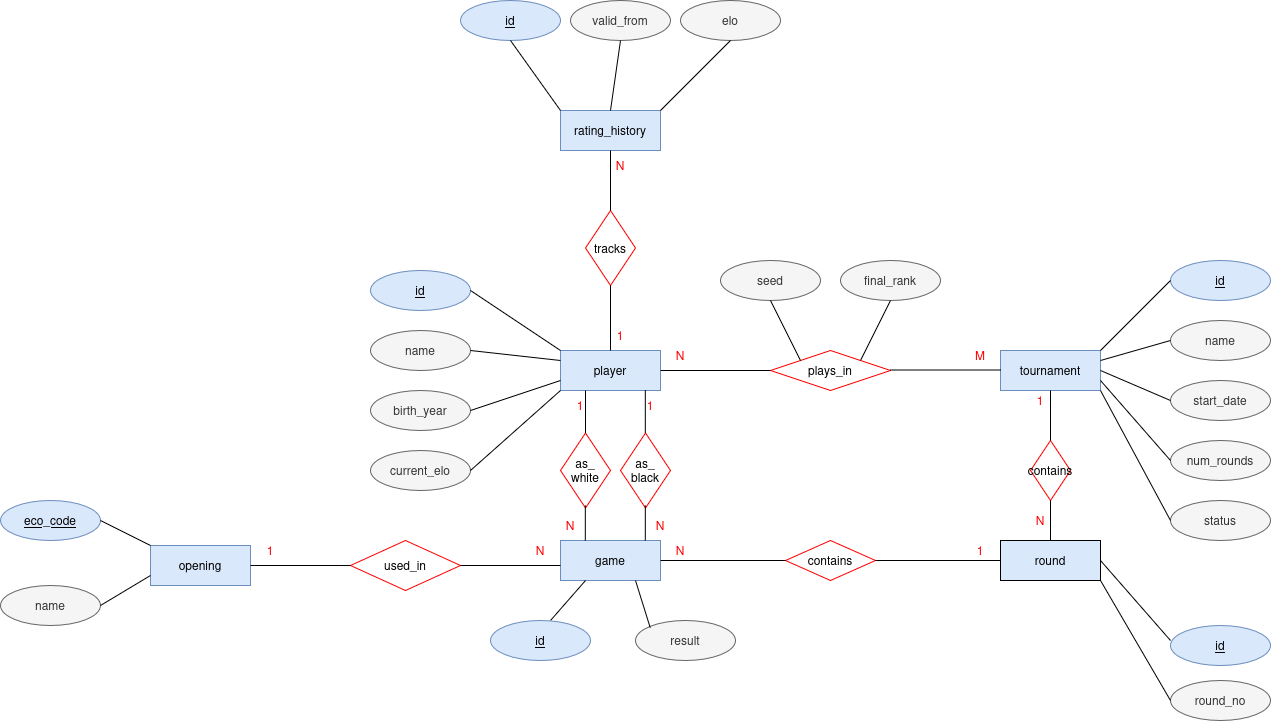
\includegraphics[width=0.85\linewidth]{assets/figure_1.png}
  \caption{ER sketch of the chess-club data model: entity types, key attributes,
  relationships and cardinalities. The central N:M relationship is
  \emph{player~$\leftrightarrow$~tournament}, realised through the associative
  entity \texttt{registration}.}
  \label{fig:er}
\end{figure}

Figure~\ref{fig:er} shows the data model. The central entity types are
\texttt{player} (name, birth year, current Elo), \texttt{tournament} (name,
start date, number of rounds, status), \texttt{round} (round number within a
tournament), \texttt{game} (linking two players and one opening within a
round, plus the result), \texttt{opening} (ECO code, name) and
\texttt{rating\_history} (Elo value of a player at a point in time). The
mandatory \textbf{N:M relationship} is
\emph{player~$\leftrightarrow$~tournament}: a player takes part in many
tournaments over time, and a tournament has many players. It is resolved by
the associative entity \texttt{registration}, which carries the seed and the
final rank. Every \texttt{game} connects two players (white and black),
belongs to exactly one round, and uses exactly one opening.
The relationship
\emph{tournament~$\rightarrow$~round~$\rightarrow$~game} is a strict 1:N chain,
and \emph{player~$\rightarrow$~rating\_history} is 1:N as well. In the final
implementation, creating a tournament also creates round numbers
\texttt{1..num\_rounds} in the same backend transaction.

% ============================================================
\section{From model to schema}
% ============================================================

Applying the ER-to-relational mapping rules to Figure~\ref{fig:er} 
yields a schema of seven tables:
each strong entity becomes a table, the N:M relationship
\texttt{plays\_in} becomes its own table \texttt{registration}
carrying the relationship attributes \texttt{seed} and
\texttt{final\_rank}, and the remaining 1:N relationships
become foreign keys on the N-side.

\begin{itemize}
  \item \texttt{player}(\underline{id}, name, birth\_year, current\_elo)
  \item \texttt{opening}(\underline{eco\_code}, name)
  \item \texttt{tournament}(\underline{id}, name, start\_date, num\_rounds, status)
  \item \texttt{registration}(\underline{\emph{player\_id}, \emph{tournament\_id}}, seed, final\_rank)
  \item \texttt{round}(\underline{id}, \emph{tournament\_id}, round\_no),
        \textsc{unique}(tournament\_id, round\_no)
  \item \texttt{game}(\underline{id}, \emph{round\_id}, \emph{white\_id}, \emph{black\_id},
        \emph{eco\_code}, result), \\
        \hspace*{1em}\textsc{check}(result IN (\texttt{'1-0'}, \texttt{'0-1'}, \texttt{'1/2-1/2'})), \\
        \hspace*{1em}\textsc{check}(white\_id $\neq$ black\_id)
  \item \texttt{rating\_history}(\underline{id}, \emph{player\_id}, valid\_from, elo)
\end{itemize}

Foreign keys: \texttt{registration.player\_id}~$\to$~\texttt{player},
\texttt{registration.tournament\_id}~$\to$~\texttt{tournament},
\texttt{round.tournament\_id}~$\to$~\texttt{tournament},
\texttt{game.round\_id}~$\to$~\texttt{round},
\texttt{game.white\_id}, \texttt{game.black\_id}~$\to$~\texttt{player},
\texttt{game.eco\_code}~$\to$~\texttt{opening},
\texttt{rating\_history.player\_id}~$\to$~\texttt{player}.

\textbf{Normalisation.} Every non-key attribute depends on the whole primary key
and only on it: opening names live in \texttt{opening}, not repeated in
\texttt{game}; a player's current Elo is stored once in \texttt{player} and its
history is factored into \texttt{rating\_history}. There are no transitive
dependencies, so the schema is in \textbf{3NF}.

% ============================================================
\section{API design}
% ============================================================
The FastAPI layer exposes four read and four write endpoints for the application.
All application endpoints require the configured \texttt{X-API-Key}; the
separate \texttt{GET /health} endpoint remains unauthenticated so service
availability can be checked independently.

\renewcommand{\arraystretch}{1.2}
\begin{tabularx}{\linewidth}{@{}p{1.6cm}p{4.6cm}X@{}}
\toprule
\textbf{Method} & \textbf{Path} & \textbf{Purpose} \\
\midrule
\texttt{GET}  & \texttt{/players}                              & list all players with name, birth year and current Elo \\
\texttt{GET}  & \texttt{/rating-history}                       & list Elo-history rows, optionally filtered by \texttt{player\_id} \\
\texttt{GET}  & \texttt{/tournaments}                          & list all tournaments \\
\texttt{GET}  & \texttt{/standings?tournament\_id=\{id\}}      & tournament standings with points, wins/draws/losses, games played and Buchholz tiebreak (\emph{JOIN + aggregation}) \\
\texttt{POST} & \texttt{/players}                              & create a player and initial rating-history row \\
\texttt{POST} & \texttt{/tournaments}                          & create a tournament and all numbered rounds atomically \\
\texttt{POST} & \texttt{/registrations}                        & register a player for a tournament with optional seed \\
\texttt{POST} & \texttt{/games}                                & record a game result and update both Elo ratings and rating history \\
\bottomrule
\end{tabularx}

The signature read endpoint is \texttt{GET /standings?tournament\_id=\{id\}}.
Its SQL query combines registrations, players, rounds and games, computes points
from recorded results and adds a full Buchholz value based on opponents' scores.
The main transactional write endpoint is \texttt{POST /games}: it validates the
players and tournament registration, inserts the game, calculates both new Elo
values with a fixed K-factor, updates \texttt{player.current\_elo} and appends
one \texttt{rating\_history} row per player. Tournament creation is also
transactional and inserts all required round rows together with the tournament.

% ============================================================
\section{Frontend prototype (hand sketches)}
% ============================================================

The frontend is a \textbf{Python/tkinter} desktop application, packaged as a
\texttt{.deb} installer as required. At startup, a connection dialog asks for
the API URL and \texttt{X-API-Key}; the frontend validates those values against
the API before opening the main application. The final application uses six
tabs: \emph{Players}, \emph{Standings}, \emph{Rating History}, \emph{Record
Game}, \emph{Register Player} and \emph{Create Tournament}. tkinter is chosen
because it ships with the Python standard library and packages cleanly into a
Debian archive.

\begin{figure}[ht]
\centering
\begin{minipage}[t]{0.47\linewidth}\centering
  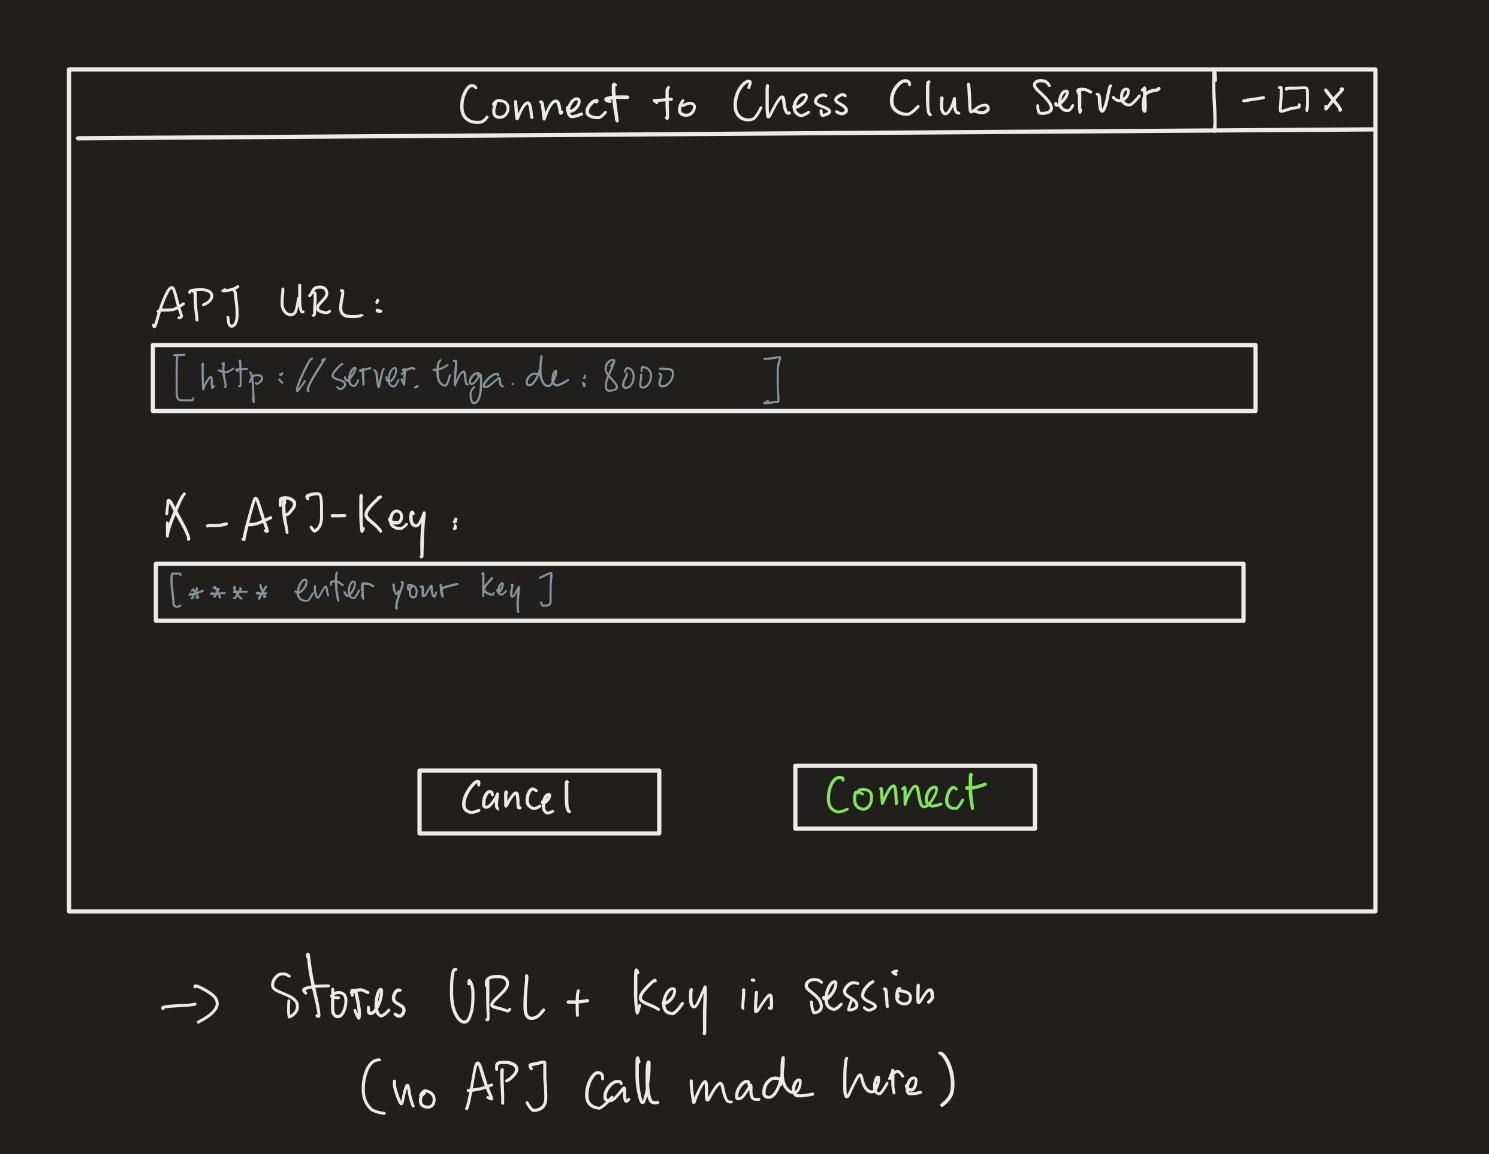
\includegraphics[width=\linewidth]{assets/figure_2.png}
  \captionof{figure}{Connection-dialog sketch; the final implementation asks for API URL and \texttt{X-API-Key} at startup.}
  \label{fig:fe-connect}
\end{minipage}\hfill
\begin{minipage}[t]{0.47\linewidth}\centering
  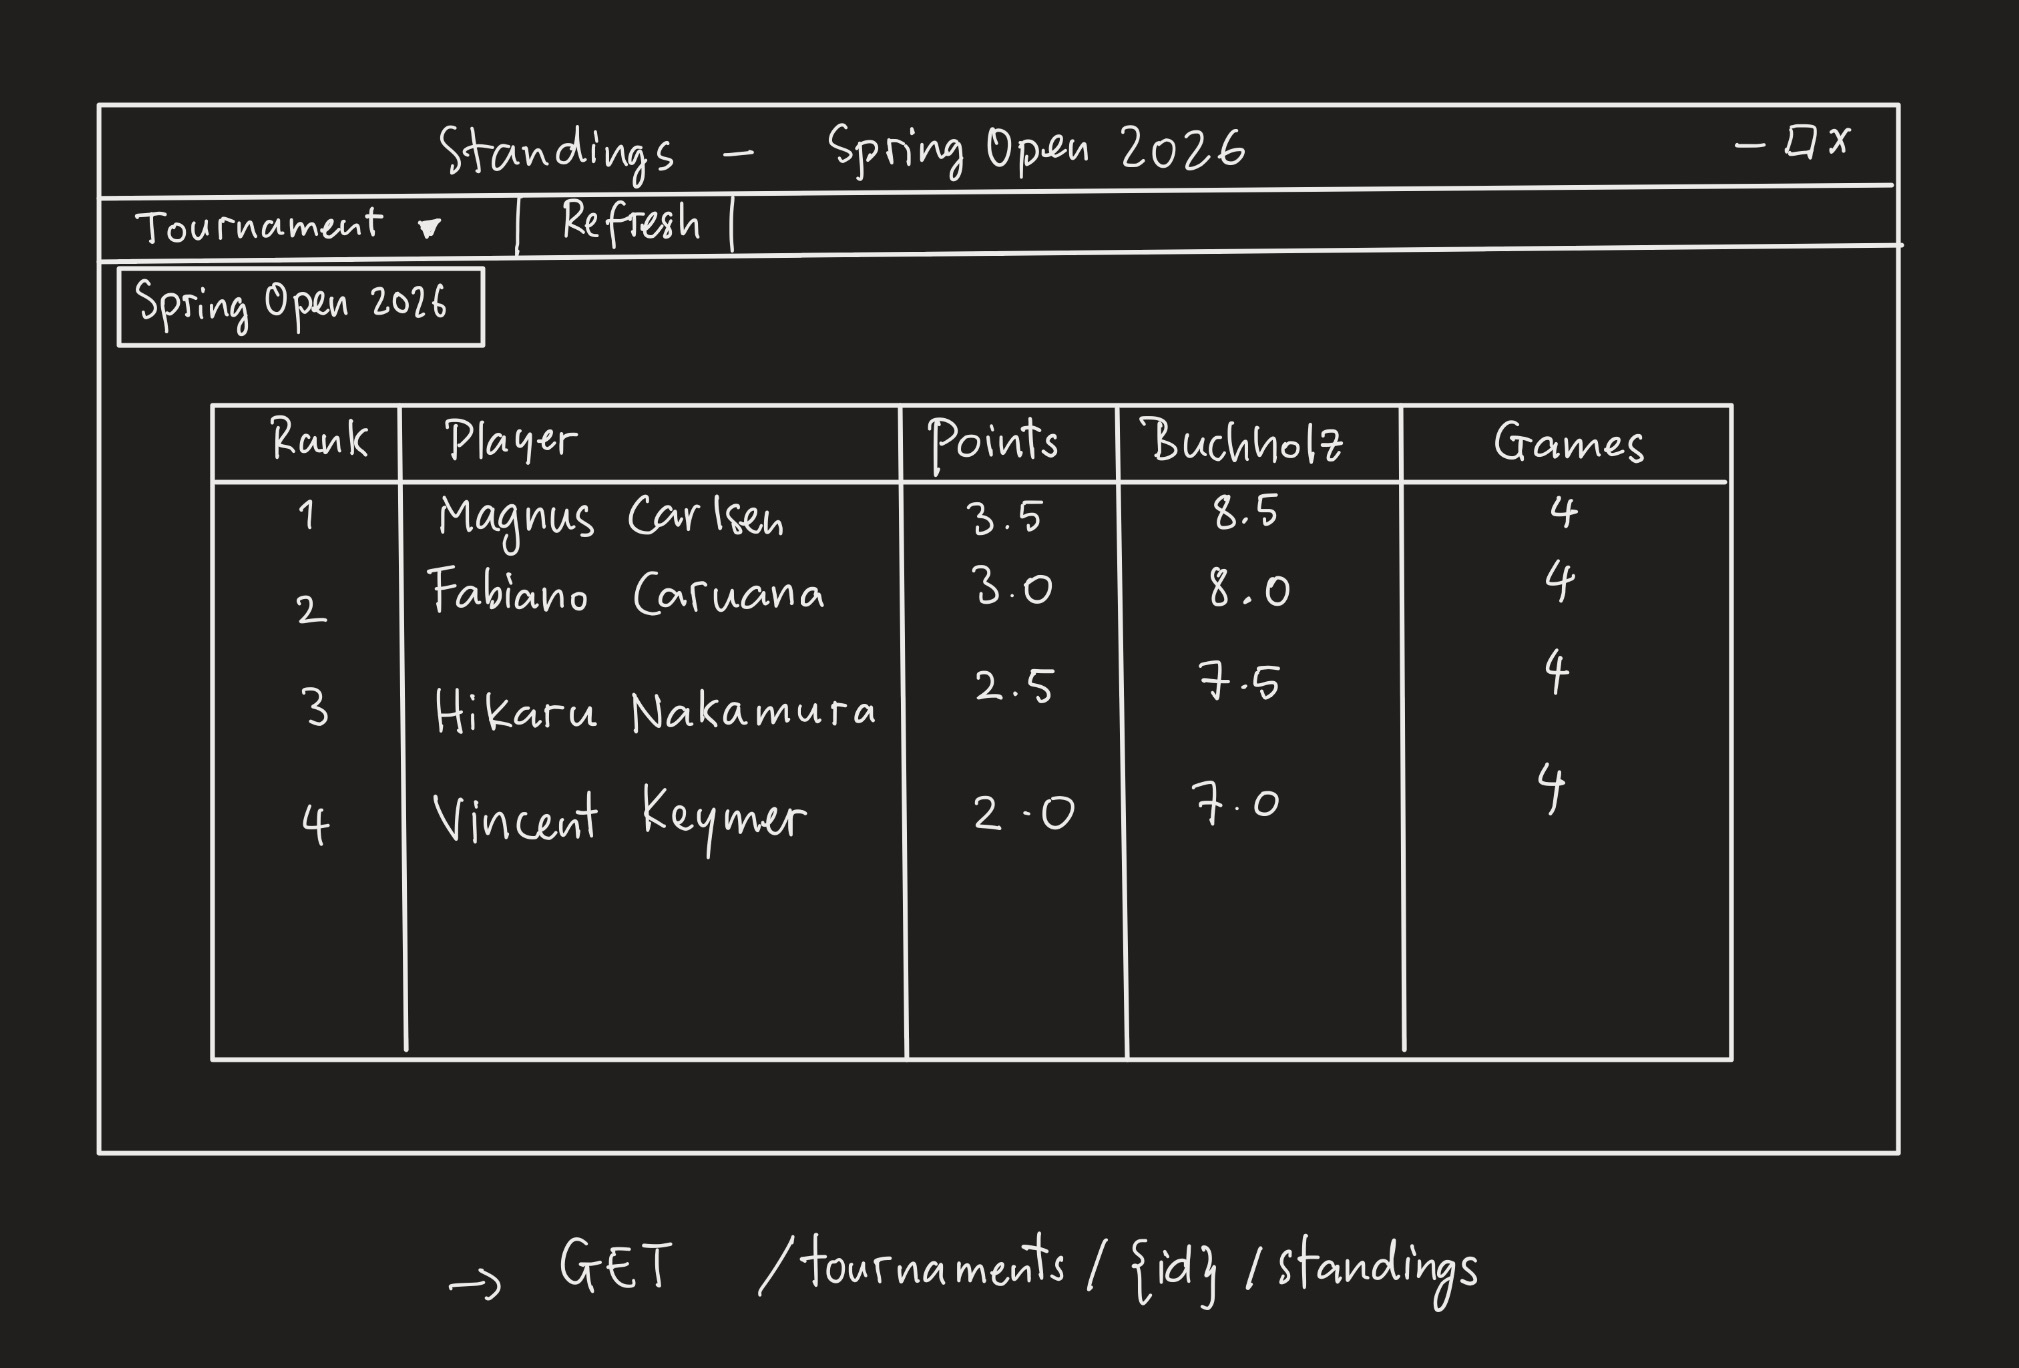
\includegraphics[width=\linewidth]{assets/figure_3.png}
  \captionof{figure}{Standings prototype; final implementation calls \texttt{GET /standings?tournament\_id=\{id\}}.}
  \label{fig:fe-main}
\end{minipage}

\vspace{1em}

\begin{minipage}[t]{0.47\linewidth}\centering
  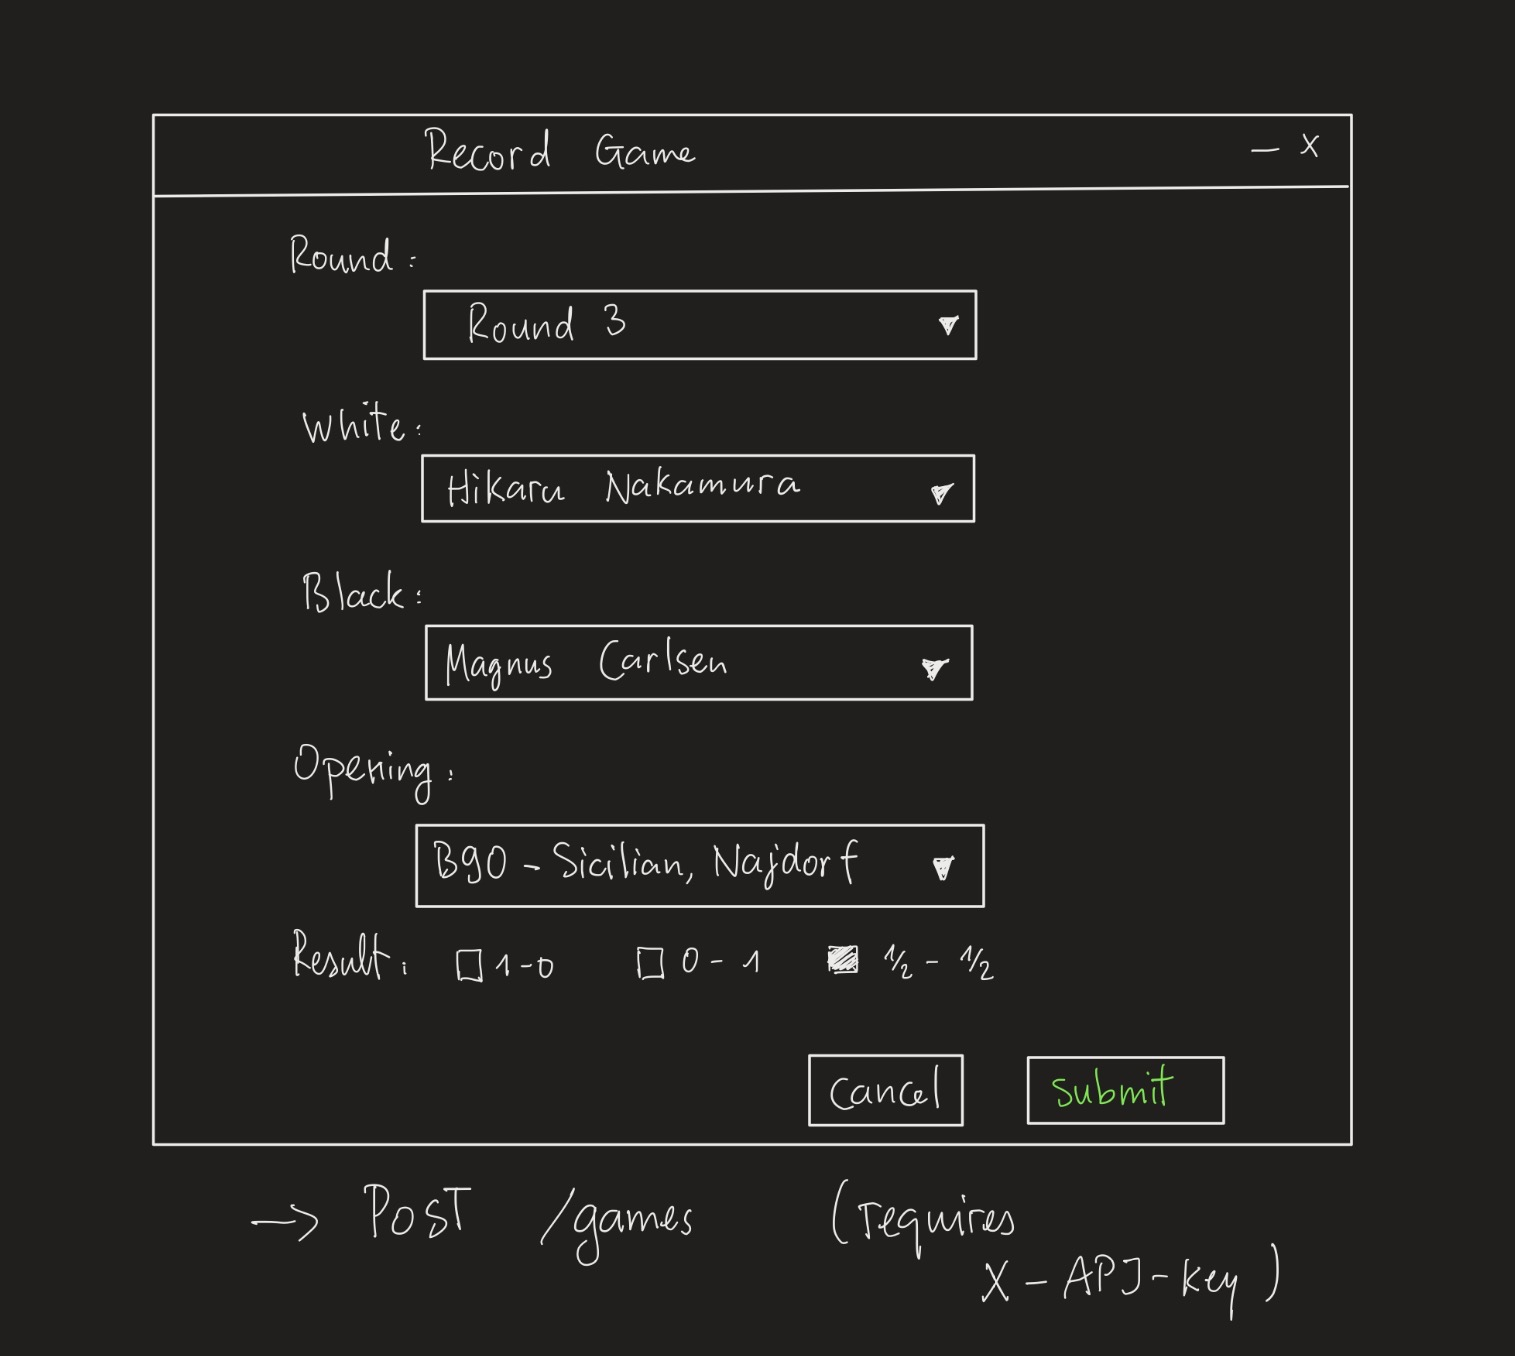
\includegraphics[width=\linewidth]{assets/figure_4.png}
  \captionof{figure}{Record-game prototype: round, white, black, opening and result -- calls \texttt{POST /games}.}
  \label{fig:fe-detail}
\end{minipage}\hfill
\begin{minipage}[t]{0.47\linewidth}\centering
  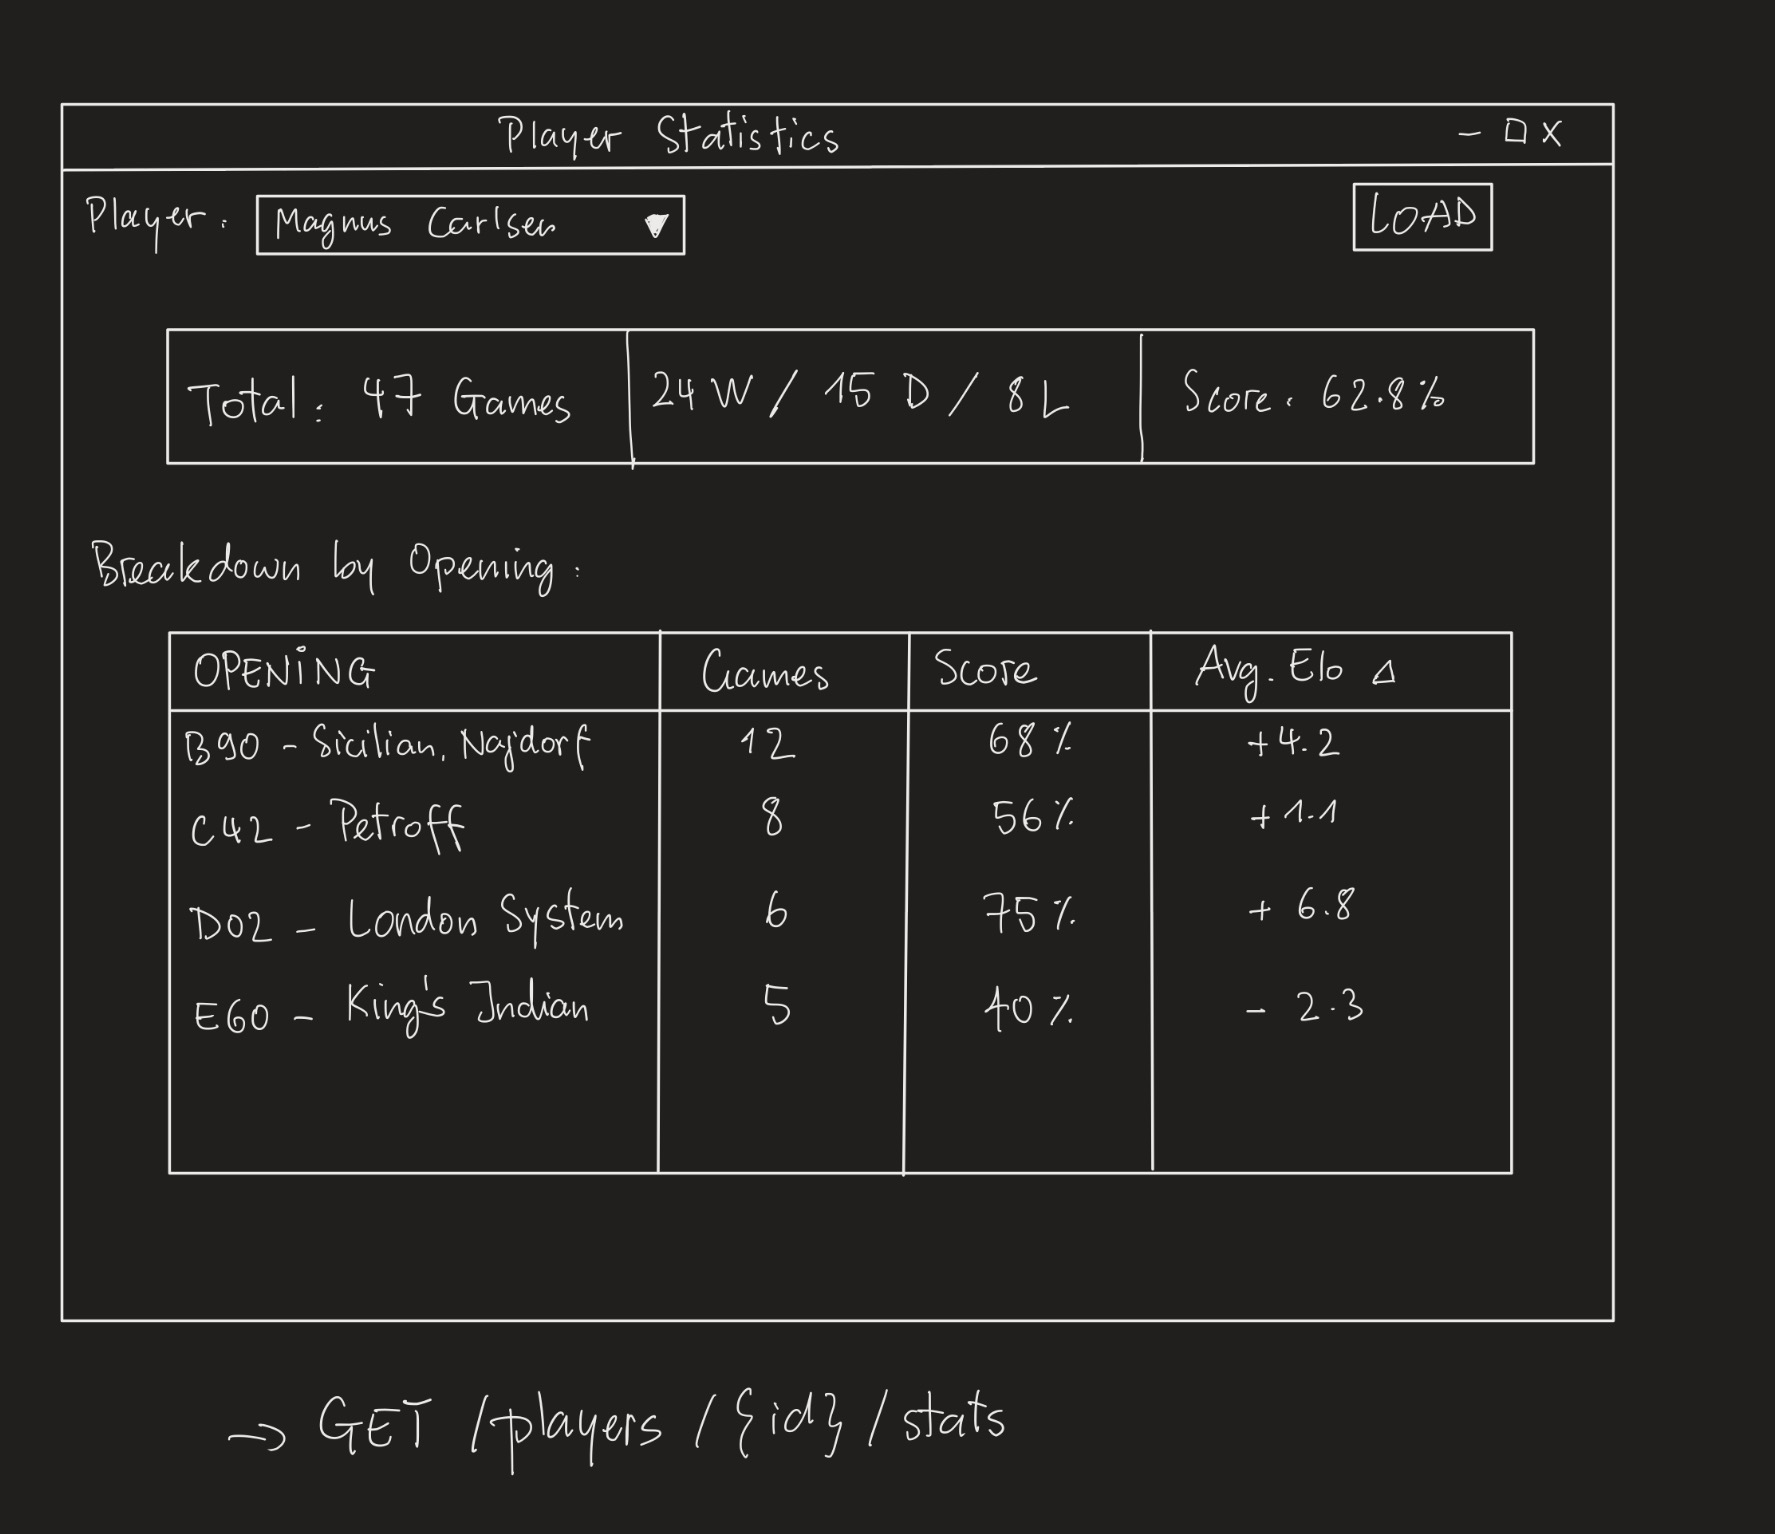
\includegraphics[width=\linewidth]{assets/figure_5.png}
  \captionof{figure}{Early player-statistics sketch; final implementation uses a dedicated Elo Rating History tab instead.}
  \label{fig:fe-second}
\end{minipage}
\end{figure}

Figures~\ref{fig:fe-connect}--\ref{fig:fe-second} are retained as the original
planning sketches. During implementation the interface was organised into a
startup connection dialog followed by a single six-tab tkinter window. The
\emph{Players} tab lists players and creates new ones; \emph{Create Tournament}
creates a tournament and displays the new round IDs; \emph{Register Player}
connects players to tournaments; \emph{Record Game} records results;
\emph{Standings} displays the calculated ranking; and \emph{Rating History}
displays all Elo-history rows or filters them by player. Successful writes
refresh the relevant read views so newly created players and tournaments become
selectable without restarting the GUI.

% ============================================================
\section{Operation with Docker Compose}
% ============================================================

The backend consists of two services in \texttt{docker-compose.yml}:
\texttt{postgres}, using the official \texttt{postgres:16} image with persistent
storage and database initialisation scripts, and \texttt{api}, built from
\texttt{api/Dockerfile}. The API container connects to PostgreSQL over Docker's
internal network using the service hostname \texttt{postgres}; both services
start together with \texttt{docker compose up -d --build}. The frontend remains
outside Docker and is delivered separately as a Debian package. Credentials and
the API key live in \texttt{.env}. This matches the required deployment model:
containerized backend plus installed desktop frontend.

% ============================================================
\section{Scope, milestones and risks}
% ============================================================

\textbf{Scope.} 7 tables, 8 application endpoints (4 read, 4 write) plus the
health endpoint, and a startup connection dialog followed by a 6-tab tkinter
frontend. Automatic Swiss pairing, player-opening analytics, user accounts,
edit/delete workflows and tournament closing are explicitly outside the final
scope.

\textbf{Milestones and schedule.}

\renewcommand{\arraystretch}{1.2}
\begin{tabularx}{\linewidth}{@{}p{1.4cm}Xp{1.8cm}@{}}
\toprule
\textbf{Week} & \textbf{Milestone} & \textbf{Est. hours} \\
\midrule
1     & Schema, DDL and seed data ready in PostgreSQL, including all seven final tables and constraints & 8 \\
2--3  & FastAPI read/write endpoints, \texttt{X-API-Key} dependency, standings/Buchholz query and Elo business logic & 12 \\
4--5  & Docker Compose backend, tkinter frontend with connection dialog and six tabs, plus \texttt{.deb} packaging & 10 \\
6     & \texttt{pytest}, Compose/database smoke tests, LaTeX documentation with CI/release automation, and 8--10 min demonstration video & 10 \\
\bottomrule
\end{tabularx}

\textbf{Risks.} (1)~The Elo update on \texttt{POST /games} is a small business
rule with real edge cases: both players' ratings must move symmetrically and
recording a game against an unregistered player must be refused. These cases
are therefore covered directly by automated tests.
(2)~Packaging the tkinter frontend as a working \texttt{.deb} remains a
build-system concern separate from the relational database itself.

% ============================================================
\section{Acceptance criteria and testing}
% ============================================================

The system counts as done and correct when the criteria below are verified by
the automated test suite and the containerized/local PostgreSQL test environments.

\textbf{Acceptance criteria.}
\begin{itemize}[topsep=2pt]
  \item A \texttt{POST /games} with \texttt{white\_id = black\_id} is rejected
        with HTTP~400.
  \item A \texttt{POST /games} whose \texttt{result} is not in
        \texttt{\{'1-0','0-1','1/2-1/2'\}} is rejected with HTTP~400.
  \item Registering the same player twice for the same tournament is rejected
        with HTTP~409 (primary key on \texttt{registration}).
  \item Recording a game for a player who is not registered in that
        tournament is rejected with HTTP~409.
  \item \texttt{GET /standings?tournament\_id=\{id\}} returns the correct
        points per player and Buchholz tiebreak using JOINs and aggregation.
  \item Every protected application endpoint without a valid
        \texttt{X-API-Key} returns HTTP~401; \texttt{GET /health} remains public.
\end{itemize}

\textbf{Test plan.}
\begin{itemize}[topsep=2pt]
  \item \textbf{Database:} PK on all tables, composite PK on
        \texttt{registration}, FKs on \texttt{round}, \texttt{game},
        \texttt{registration}, \texttt{rating\_history}, \textsc{unique} on
        \texttt{(tournament\_id, round\_no)}, \textsc{check} on
        \texttt{game.result} and on \texttt{white\_id $\neq$ black\_id},
        \textsc{not null} on all foreign keys; CI also applies schema and seed
        data to PostgreSQL~16 and verifies expected row counts.
  \item \textbf{API:} \texttt{pytest} with FastAPI's \texttt{TestClient}
        against an isolated PostgreSQL test database. Happy paths cover the
        implemented read and write endpoints, including player creation,
        tournament creation with automatic rounds, registration, game recording,
        rating-history filtering and standings, plus the documented 4xx cases.
  \item \textbf{Deployment:} CI builds the API image, starts PostgreSQL and the
        FastAPI service with Docker Compose, and verifies the public health
        endpoint. It also builds and inspects the Debian frontend package.
  \item \textbf{Business rule (risk 1).} Dedicated tests assert HTTP~409 for an
        unregistered player; a legal game must update both players' Elo values
        symmetrically and write one \texttt{rating\_history} row for each.
        Tournament-creation tests also verify that exactly the requested numbered
        rounds are created and that zero rounds is rejected.
\end{itemize}

\vspace{1em}
\begin{infobox}
\textbf{Effort budget:} the whole term project (system, documentation and video)
fits into roughly \textbf{40\,h of work} over at most \textbf{2 months}. The
milestone table above sums to exactly that budget.
\end{infobox}

\end{document}